\documentclass[11pt]{article}
\usepackage{amsmath, amssymb, amsthm}
\usepackage[retainorgcmds]{IEEEtrantools}

\usepackage{tikz}
\usetikzlibrary{intersections, decorations.pathreplacing}

%Listings stuff
\usepackage{listings}
\usepackage{lstautogobble}
\usepackage{color}

\definecolor{gray}{rgb}{0.5,0.5,0.5}
\lstset{
basicstyle={\small\ttfamily},
tabsize=3,
numbers=left,
numbersep=5pt,
numberstyle=\tiny\color{gray},
stepnumber=2,
breaklines=true,
boxpos=t
}

\usepackage{fancyhdr}

%Format stuff
\pagestyle{fancy}
\headheight 35pt

%Header info
\chead{\Large \textbf{Greedy Scheduling Algorithms}}
\lhead{}
\rhead{}

\begin{document}

\section{Interval Scheduling}

	\begin{description}
		\item[Input:] A set of requests $R$ for a resources, where $\forall r \in R$, there is a start time $s_i$ and finish time $f_i$.
		\item[Output:] A subset of $R$ with no conflicts that maximizes the number of scheduled events.
	\end{description}
	
	\subsection{Greedy Criterion}
		A number of schemes are possible for the algorithm, including shortest request first, earliest start time first, and earliest finish time first.
		
		Shortest request is suboptimal from the following counterexample, where it would schedule two requests instead of the optimal 3. By extrapolating this principle, shortest request could be off by a factor of 2 from the optimal schedule because one request can conflict with 2 optimal requests.
		\begin{center}
		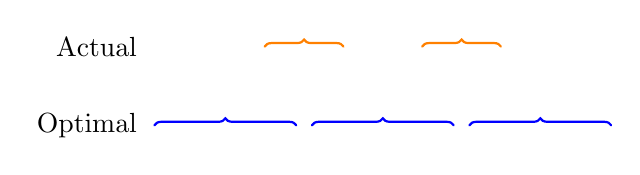
\begin{tikzpicture}
			[scale=1,line cap=round,
			%Styles
			axes/.style=,
			important line/.style={very thick},
			information text/.style={rounded corners,fill=red!10,inner sep=1ex},
			dot/.style={circle,inner sep=1pt,fill,label={#1},name=#1}			
			]
			
			%Colors
			\colorlet{anglecolor}{green!50!black}	%angle arcs/lines
			
			%The graphic
			
			\node[left] at (0, 0) {Actual};
			\node[left] at (0, -1) {Optimal};
			
			\draw[decorate,decoration=brace,blue,thick] (.1, -1) -- (1.9, -1);
			\draw[decorate,decoration=brace,blue,thick] (2.1, -1) -- (3.9, -1);
			\draw[decorate,decoration=brace,blue,thick] (4.1, -1) -- (5.9, -1);
			
			\draw[decorate,decoration=brace,orange,thick] (1.5, 0) -- (2.5, 0);
			\draw[decorate,decoration=brace,orange,thick] (3.5, 0) -- (4.5, 0);
		\end{tikzpicture}
		\end{center}
		
		Earliest start time is actually a horrible criterion, as demonstrated by the following counterexample:
		
		\begin{center}
		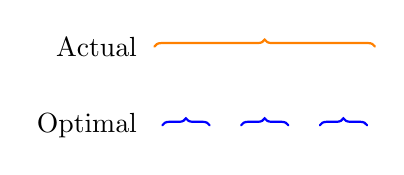
\begin{tikzpicture}
			[scale=1,line cap=round,
			%Styles
			axes/.style=,
			important line/.style={very thick},
			information text/.style={rounded corners,fill=red!10,inner sep=1ex},
			dot/.style={circle,inner sep=1pt,fill,label={#1},name=#1}			
			]
			
			%Colors
			\colorlet{anglecolor}{green!50!black}	%angle arcs/lines
			
			%The graphic
			
			\node[left] at (0, 0) {Actual};
			\node[left] at (0, -1) {Optimal};
			
			\draw[decorate,decoration=brace,blue,thick] (.2, -1) -- (.8, -1);
			\draw[decorate,decoration=brace,blue,thick] (1.2, -1) -- (1.8, -1);
			\draw[decorate,decoration=brace,blue,thick] (2.2, -1) -- (2.8, -1);
			
			\draw[decorate,decoration=brace,orange,thick] (.1, 0) -- (2.9, 0);
		\end{tikzpicture}
		\end{center}
		
		In the end, the optimal greedy criterion is actually sorting requests by earliest finish time, because it frees up the shared resource ASAP. Note this can be implemented in $\Theta(n)$ time by one walkthrough of the list - pick the first valid element, then walk along the list until the next valid start time, and so on.
		
	\subsection{Proof}
		Let $O$ be some optimal schedule and $G$ be the greedy schedule generated by the algorithm such that $O = G$ up to some index $j$. From our greedy criterion, we know that $f_j^G \leq f_j^O$. Therefore, we can swap $O_j$ with $G_j$ without introducing any more conflict, producing a new still-optimal schedule $O'$.
		
		By induction, it is possible to transform any optimal schedule into our greedy schedule while maintaining optimality. Therefore, the greedy algorithm produces an optimal schedule.
		
\section{Interval Coloring}
	\begin{description}
		\item[Input:] Set of requests $R(s_i, f_i)$.
		\item[Output:] A minimum coloring of requests such that there is no conflict within a color.
	\end{description}
		
		\subsection{Greedy Criterion}
			The greed criterion for this algorithm is actually quite straightforward - assign the smallest non-conflicting color to the next activity sorted by start time.
			
			\begin{lstlisting}[autogobble=true,mathescape]
				for $r_i$ $\in$ R:
					for $r_j$ $\in$ R $\mid$ j < i:
						if $r_j$ conflicts with $r_i$:
							exclude color of $r_j$
							
					if $\exists$ color not excluded:
						assign color to $r_i$
					else:
						leave $r_i$ uncolored
			\end{lstlisting}
		
		\subsection{Proof}
			Define $d$ as the depth of the set of requests $R$, or the maximum number of conflicting requests at some point in time.
			
			\subparagraph{Claim:} No interval ends up unlabeled, and only $d$ colors are used.
			
			\subparagraph{Proof:} Consider one of the requests $r_i$, and suppose there are $t$ requests earlier in the sorted order that conflict with it. This means that the depth at some point in $r_i$ is $t + 1$, which, given our definition of $d$, means $t + 1\leq d$ and so $t \leq d - 1$. It follows then that if we use $d$ labels, at least 1 will be free to color. Extending this analysis also proves that exactly $d$ colors are used.
			
			Because the algorithm by design never assigns conflicting requests to the same color and only uses $d$ colors total, it produces the optimal coloring of requests.
		
\section{Minimizing Lateness}
	\begin{description}
		\item[Input:] A set of tasks $T(t_i, d_i)$ where $t_i$ is the duration of a task and $d_i$ is the deadline.
		\item[Output:] A schedule of tasks that minimizes the maximum amount of time that a task overshoots its deadline.
	\end{description}	
	
	\subsection{Greedy Criterion}
		Counterintuitively, we get the best result by sorting by earliest deadlines first. Even though half of the input is ignored, this scheme still produces an optimal schedule.
		
	\subsection{Proof}
		\subparagraph{Claim:} The greedy algorithm does not have any \textit{idle time} - when there are jobs left but the machine is not working - and there exists an optimal schedule with no idle time. Both these points are obvious.
		
		Now define an \textit{inversion} in a schedule as a job $i$ with deadline $d_i$ is scheduled before a job $j$ with deadline $d_j < d_i$. By definition, the greedy schedule has no inversions. 
		
		\subparagraph{Claim:} All schedules with no inversions and no idle time have the same maximum lateness.
		
		\subparagraph{Proof:} If 2 schedules have no inversions or idle time, then they can only differ in the order in which jobs with identical deadlines are scheduled. Consider some deadline $d$ such that in both schedules, the jobs with deadline $d$ are all scheduled consecutively. Among the jobs with this deadline, the last one has the greatest lateness, the sum of all durations of these jobs, which does not depend on the order.
		
		Now suppose there exists some optimal schedule $O$ with no idle time but with inversions - that is, there is a pair of jobs $i, j$ such that $j = i + 1$ and $d_j < d_i$. The greedy schedule $G$ is identical to $O$ up to the first task in this pair, but $G$ has no inversions.
		
		Let $l_i^O, l_j^O$ be the lateness of $O_i, O_j$, and $l_i^G, l_j^G$ be lateness of $G_i, G_j$. Let $t$ be the common start time between the two schedules for tasks $i$ and $j$. It's easy to see that, given a non-negative lateness,
		
		\begin{IEEEeqnarray}{rCl}
			l_i^O & = & t + t_i - d_i\\
			l_j^O & = & t + (t_i + t_j) - d_j
		\end{IEEEeqnarray}
		
		and similarly for $G$,
		
		\begin{IEEEeqnarray}{rCl}
			l_i^G & = & t + (t_i + t_j) - d_i\\
			l_j^G & = & t + t_j - d_j
		\end{IEEEeqnarray}
		
		By definition of an inversion, we know that $d_j < d_i$, and because a task must have non-negative duration,
		
		\begin{equation}
			l_j^O = t + (t_i + t_j) - d_j > t + t_i - d_i = l_i^O
		\end{equation}
		Therefore, the maximum lateness of $O$ for this inversion is $L^O = l_j^O$.
		
		A similar analysis for lateness in $G$ shows that
		\begin{IEEEeqnarray}{rCl}
			l_i^G & = & t + (t_i + t_j) - d_i < t + (t_i + t_j) - d_j = L^O\\
			l_j^G & = & t + t_j - d_j \leq t + t_i + t_j - d_j = L^O
		\end{IEEEeqnarray}
		
		Therefore, no matter if $L^G = l_i^G$ or $L^G = l_j^G$, $L^G \leq L^O$, so tasks $i$ and $j$ in $O$ can be exchanged without increasing the maximum lateness. By induction then we can turn any optimal schedule $O$ with inversions into a greedy schedule $G$ without inversions by flipping all inversions in $O$, so therefore the algorithm produces an optimal schedule.

\section{Cache Scheduling}
	\begin{description}
		\item[Input:] A list of jobs $j$ each with a weight $w_j$ and length $l_j$.
		\item[Output:] An ordering of jobs that minimizes the weighted sum of completion times, where completion time is the amount of wall time it takes from the beginning to the completion of job $j$.
		\[C_j = \sum_1^j l_j\]
		\[min(\sum_1^nw_jC_j)\]
	\end{description}
	
\subsection{Greedy Criterion}
	\subsubsection{Special Cases}
		\subparagraph{Identical lengths} In this case, we choose the larger-weight jobs first to minimize the term in the sum (when $n$ is smaller).
			\begin{equation}
				\sum_1^n w_jC_j = \sum_1^n w_j \cdot n \cdot L = L \cdot \sum_1^n w_j \cdot n
			\end{equation}
		\subparagraph{Identical weights} In this case, we choose the shortest jobs first to minimize the sum over completion times.
			\begin{equation}
				\sum_1^n WC_j = W\sum_1^n C_j
			\end{equation}
			
	\subsubsection{Resolving Conflicting Advice}
		The key idea is to assign each job a score that is directly proportional with $w$ and indirectly proportional with $l$. Taking two guesses at such a score, there are 
		\begin{itemize}
			\item $s_j = w_j - l_j$
			\item $s_j = w_j / l_j$
		\end{itemize}
		To distinguish between the two, find the simplest example that produces different outputs. In this case, for the two jobs $j_1(w=3, l=5), j_2(w=1,l=2)$, the second score yields the lower weighted sum, so it is better than the first.
		
\section{Proof}
	\begin{description}
		\item[Claim:] sorting by decreasing ratio $w_j / l_j$ is always correct
		\item[Proof:] by exchange argument and contradiction.
		\item[Assume:] no ties in ratios (doesn't change algorithm, only proof)
	\end{description}
	
	Fix an arbitrary input of $n$ jobs with $\sigma$ as the greedy schedule from the algorithm and $\sigma^*$ being a theoretically optimal algorithm. Next, rename the jobs $j_1, j_2, \ldots , j_n$ such that $s_1 > s_2 > \ldots > s_n$, so that $\sigma$ just involves ordering the jobs in numerical order.
	
	Assuming $\sigma^* \neq \sigma$, there must exist two consecutive jobs $(i, j) \in \sigma^* \mid i > j$. Because $\sigma$ is a unique schedule (properly ordered), the only way $\sigma^*$ can be different is if at least one pair of jobs is flipped.
	
	Suppose we exchange the order of these two jobs in $\sigma^*$, leaving all other jobs unchanged. Jobs other than these two have no impact on completion time after this operation, while $C_i$ increases and $C_j$ decreases.
	
	\begin{IEEEeqnarray}{rCl}
		i > j & \rightarrow & \frac{w_i}{l_i} < \frac{w_j}{l_j}\\
		&& w_i l_j < w_j l _i
	\end{IEEEeqnarray}
	
	From the definition of weighted sum, it's clear that the cost associated with this exchange is outweighed by the benefit. Therefore, it is impossible for $\sigma^*$ to be optimal, violating out assumption in the first step, so $\sigma$ is an optimal schedule.
%	\begin{center}
%	\begin{tikzpicture}
%		[scale=3,line cap=round,
%		%Styles
%		axes/.style=,
%		important line/.style={very thick},
%		information text/.style={rounded corners,fill=red!10,inner sep=1ex},
%		dot/.style={circle,inner sep=1pt,fill,label={#1},name=#1}			
%		]
%		
%		%Colors
%		\colorlet{anglecolor}{green!50!black}	%angle arcs/lines
%		
%		%The graphic
%	\end{tikzpicture}
%	\end{center}

%	\begin{figure}[htb]
%		\centering
%		\includegraphics[width=0.8\textwidth]{filename.eps}
%		\caption{Caption.}
%		\label{fig:figure}
%	\end{figure}

%		\def\enotesize{\normalsize}
%		\theendnotes
\end{document}